\section{Upcoming challenges and conclusion}
\subsection{Upcoming challenges}
\begin{frame}[t]
  \frametitle{Outlook}
  \begin{columns}[T]
    \begin{column}{0.45\textwidth}
      \begin{block}{Calibration}
        A MCP is subject to ageing: the gain decreases over time.
        \begin{itemize}
          \item An uniform VUV ($<200\,\mathrm{nm}$) light irradiates the MCP input surface
          \item The MCP response is recorded by camera revelling non uniform area.
          \item The new calibration map is applied on beam images.
        \end{itemize}
      \end{block}
    \end{column}
    \begin{column}{0.45\textwidth}
      \begin{center}
        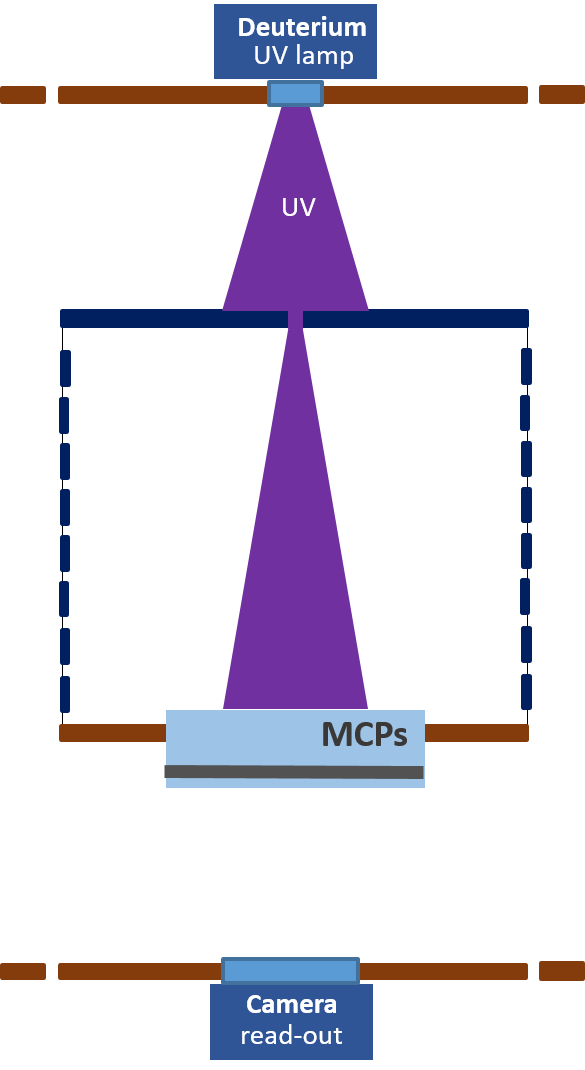
\includegraphics[width=0.5\textwidth]{05_Conclusion/fig/fig000_UV_calib}
      \end{center}
    \end{column}
  \end{columns}
  \begin{columns}[T]
    \begin{column}{0.60\textwidth}
      \vspace{0.25cm}
      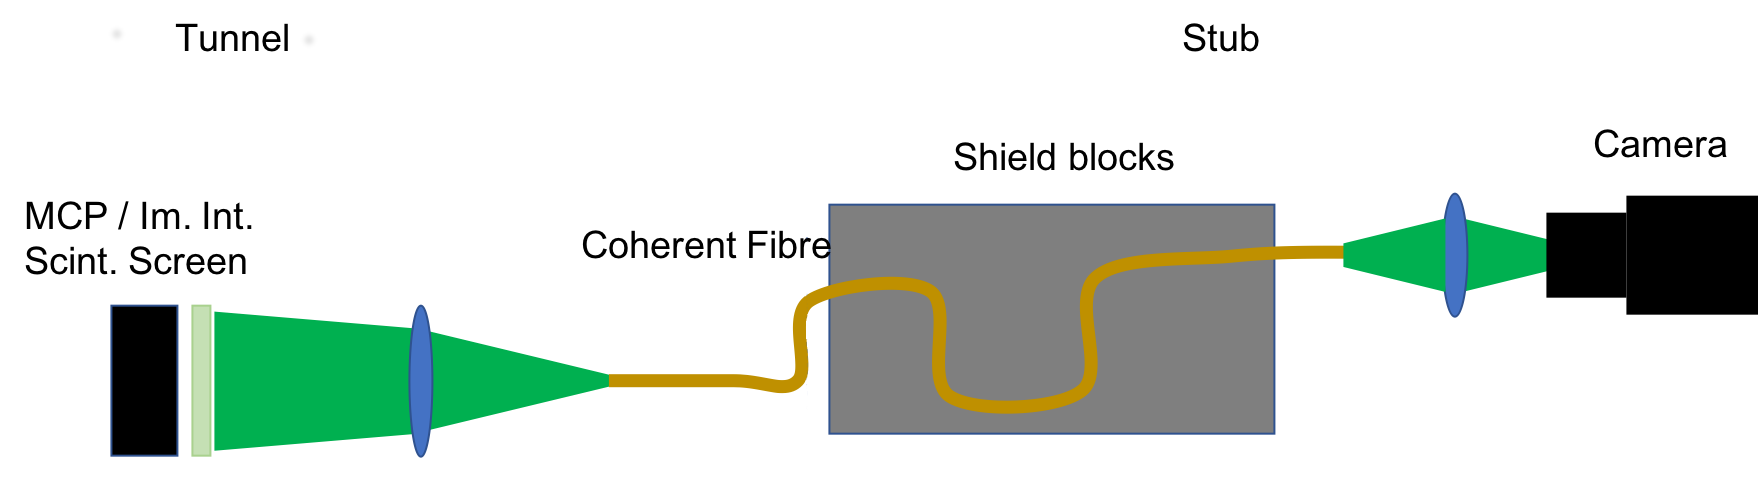
\includegraphics[width=1\textwidth]{05_Conclusion/fig/fig000_schematic_coherentr_fiber}
    \end{column}
    \begin{column}{0.35\textwidth}
      \begin{block}{Remote acquisition}
        \begin{itemize}
          \item[+] Move camera away
          \item[-] Signal and resolution decreased
        \end{itemize}
      \end{block}
    \end{column}
  \end{columns}
\end{frame}

\begin{frame}[t]
  \frametitle{Background simulation}
  \begin{block}{Background information}
    What happens if a "lost proton" hits MCP or structures around? $\implies$ simulations:
    \begin{itemize}
      \item Realistic geometry $\rightarrow$ CAD import.
      \item Information about particles.
    \end{itemize}
  \end{block}
  \begin{columns}[T]
    \begin{column}{0.45\textwidth}
      \begin{block}{Simulation with Geant4 10.X}
        Features:
        \begin{itemize}
          \item STL import.
          \item MT + MPI features.
          \item SD + ROOT output.
        \end{itemize}
        To do:
        \begin{itemize}
          \item Keep the geometry up to date.
          \item I/O with ESS particle files.
        \end{itemize}
      \end{block}
    \end{column}
    \begin{column}{0.45\textwidth}
      Example with a dummy $2\,\mathrm{GeV}$ proton hitting an IPM frame
      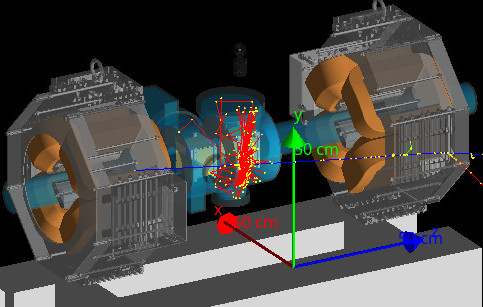
\includegraphics[width=1\textwidth]{05_Conclusion/fig/fig000_G4ESS2}
    \end{column}
  \end{columns}
\end{frame}

\begin{frame}[t]
  \frametitle{Outlook}
  \begin{columns}[T]
    \begin{column}{0.45\textwidth}
      \begin{block}{Improved design for MCP usage}
        \begin{itemize}
          \item CF200 sustains the IPM cage, should not be moved.
          \item CF160 sustains the MCP systems for replacement.
        \end{itemize}
      \end{block}
      \begin{block}{Production}
        \begin{itemize}
          \item Compliant with superconducting cavities.
          \item Production in ISO5 cleanroom
          \item Close collaboration with the IRFU cryomodule team
        \end{itemize}
      \end{block}
    \end{column}
    \begin{column}{0.45\textwidth}
      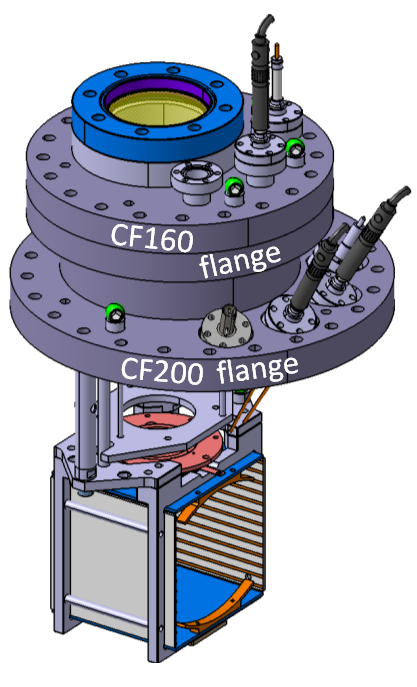
\includegraphics[width=0.75\textwidth]{05_Conclusion/fig/fig000_bride_double2_a}
    \end{column}
  \end{columns}
  \begin{block}{Production is already ongoing}
    And first IPM will be delivered in the beginning of 2020.
  \end{block}
\end{frame}

\subsection{Conclusion}
\begin{frame}[t]
  \frametitle{Conclusion}
    \begin{columns}[T]
      \begin{column}{0.45\textwidth}
        \begin{block}{In 3 years:}
          \begin{itemize}
            \item[\checkmark] The feasibility has been checked by simulations.
            \item[\checkmark] Different IPMs have been tested in real beam conditions at IPHI.
            \item[\checkmark] Both IPMs work but MCP is forseen.
          \end{itemize}
        \end{block}
        \begin{block}{Upcoming challenges:}
          \begin{itemize}
            \item Design of final version.
            \item Simulation improvement with background estimations.
            \item MCP calibration and readout.
            \item IPM production.
            \item Installation at ESS.
          \end{itemize}
        \end{block}
      \end{column}
      \begin{column}{0.45\textwidth}
      \end{column}
    \end{columns}

    \begin{textblock*}{2.8cm}(6.2cm,2cm)      
      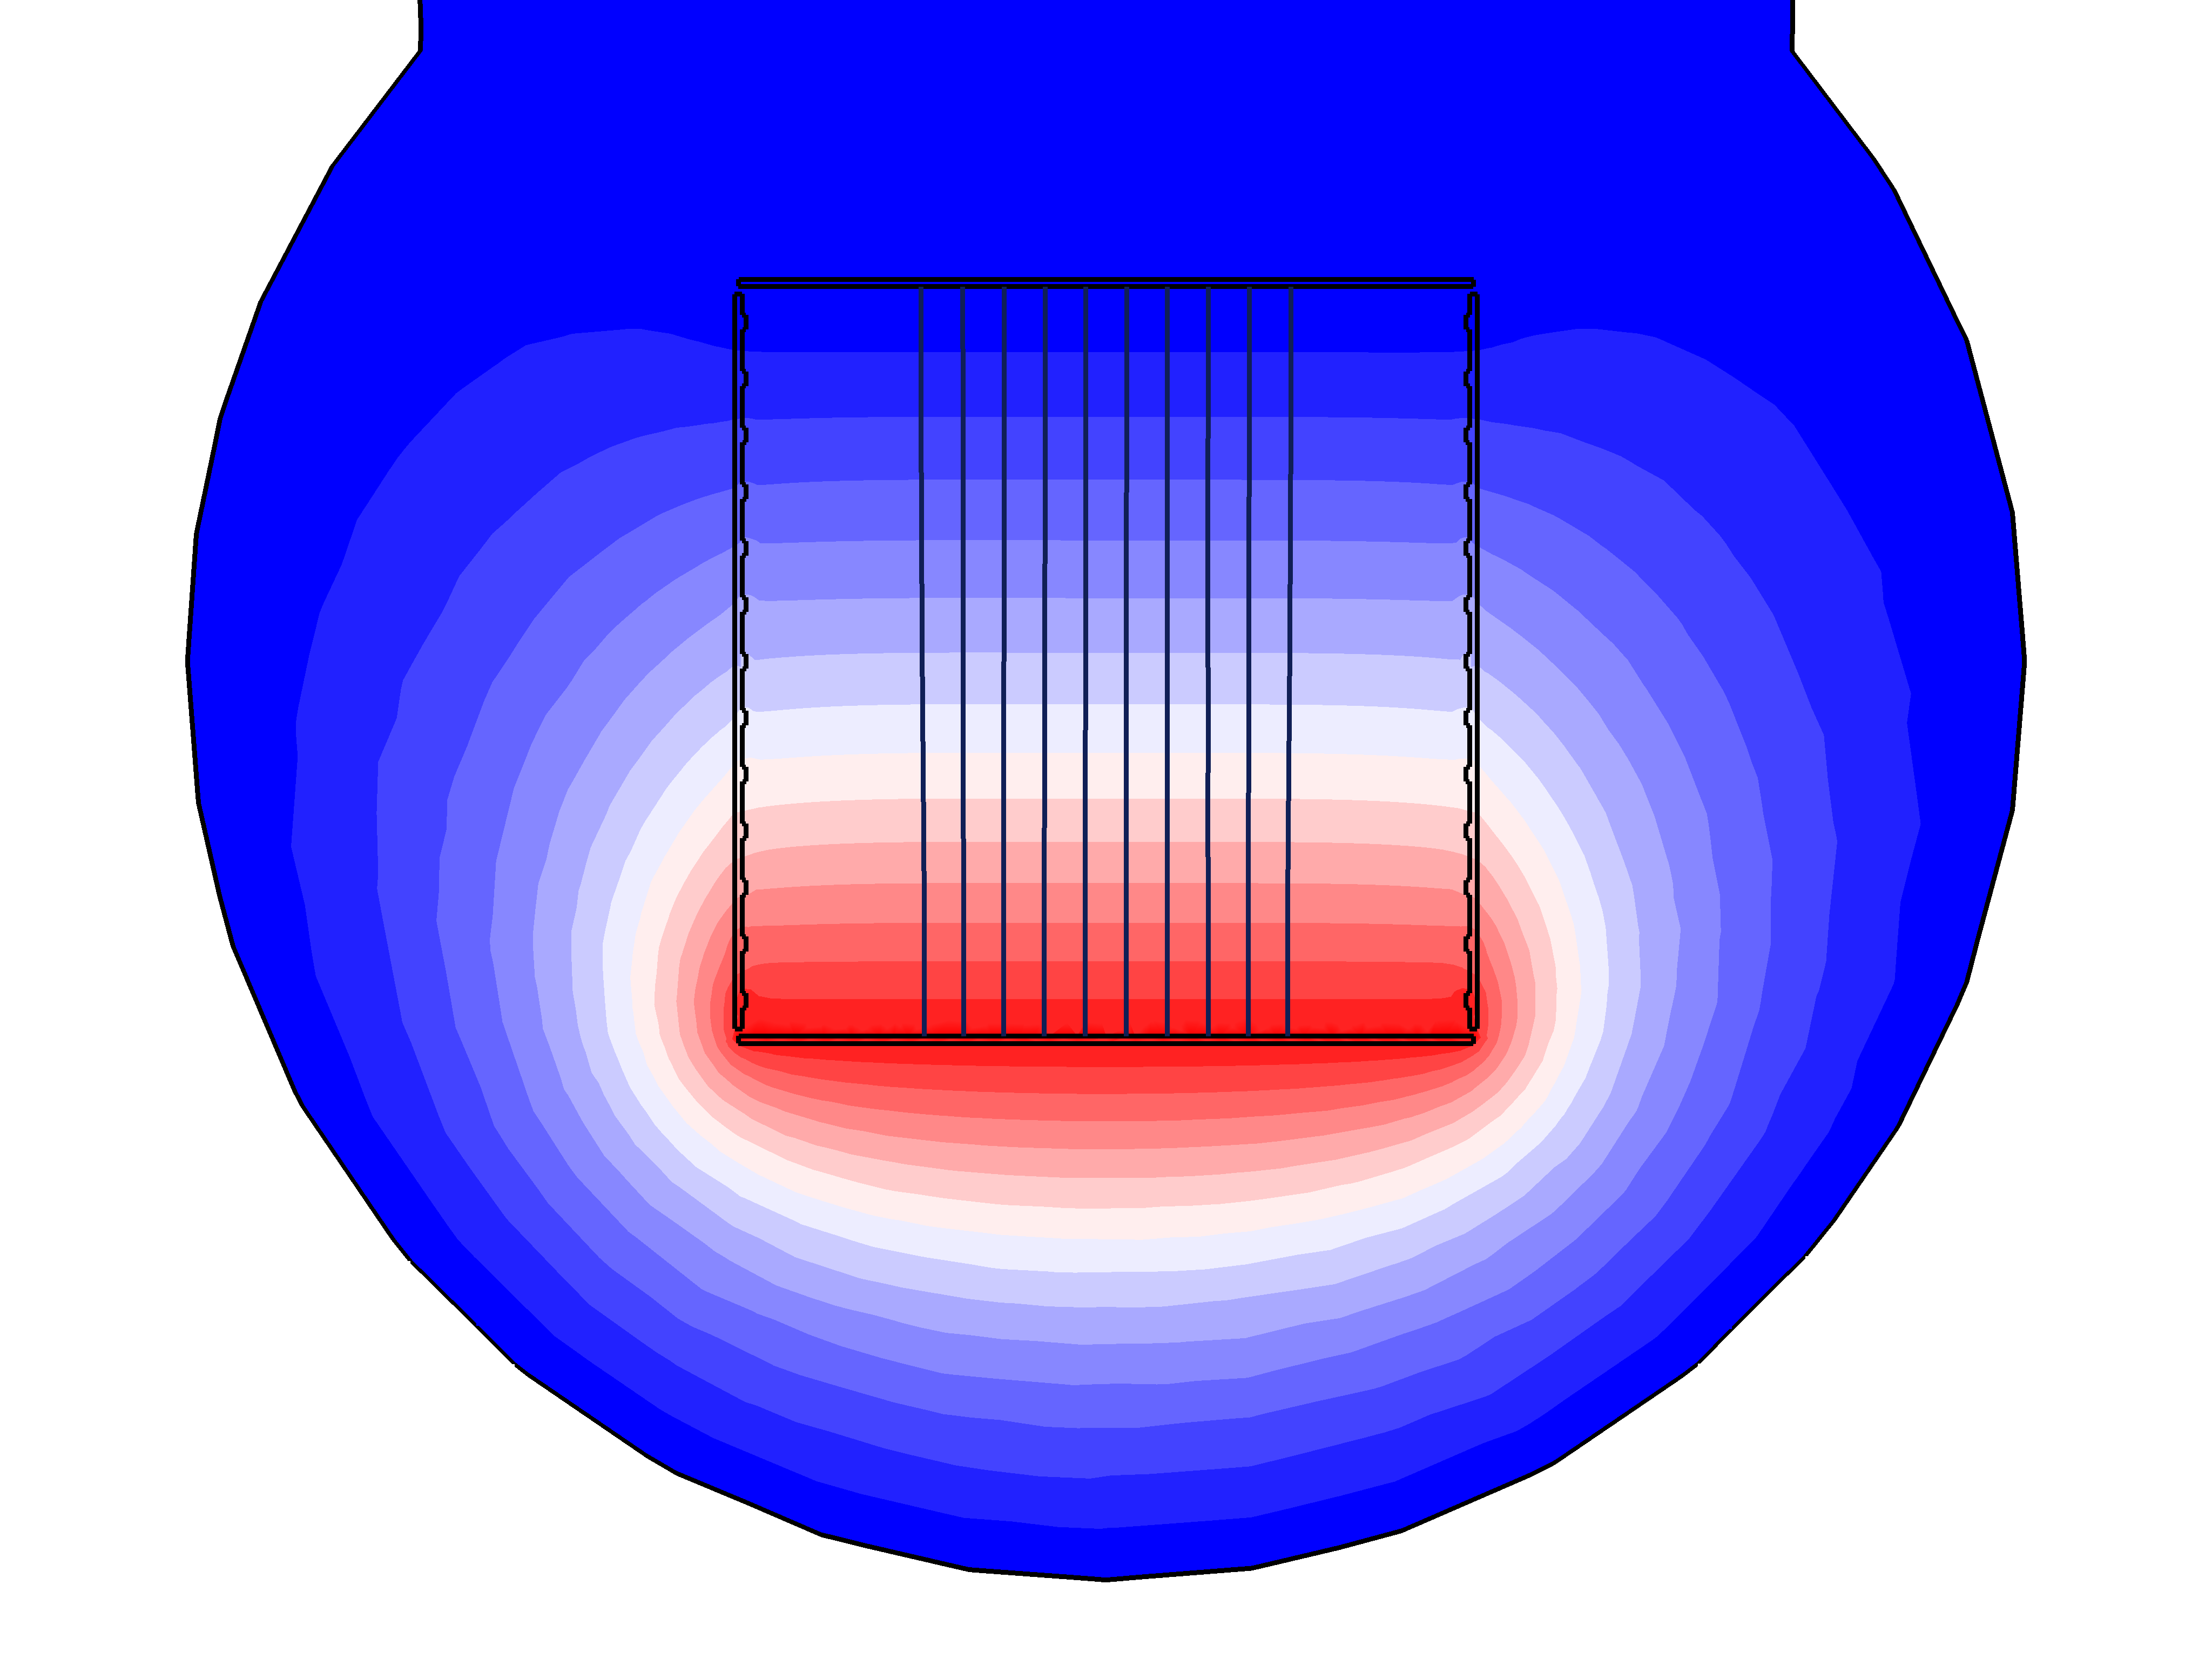
\includegraphics[width=2.8cm]{03_SIM/fig/fig000_Lines_Corr.png}
    \end{textblock*}
    \begin{textblock*}{4cm}(9cm,1.25cm)      
      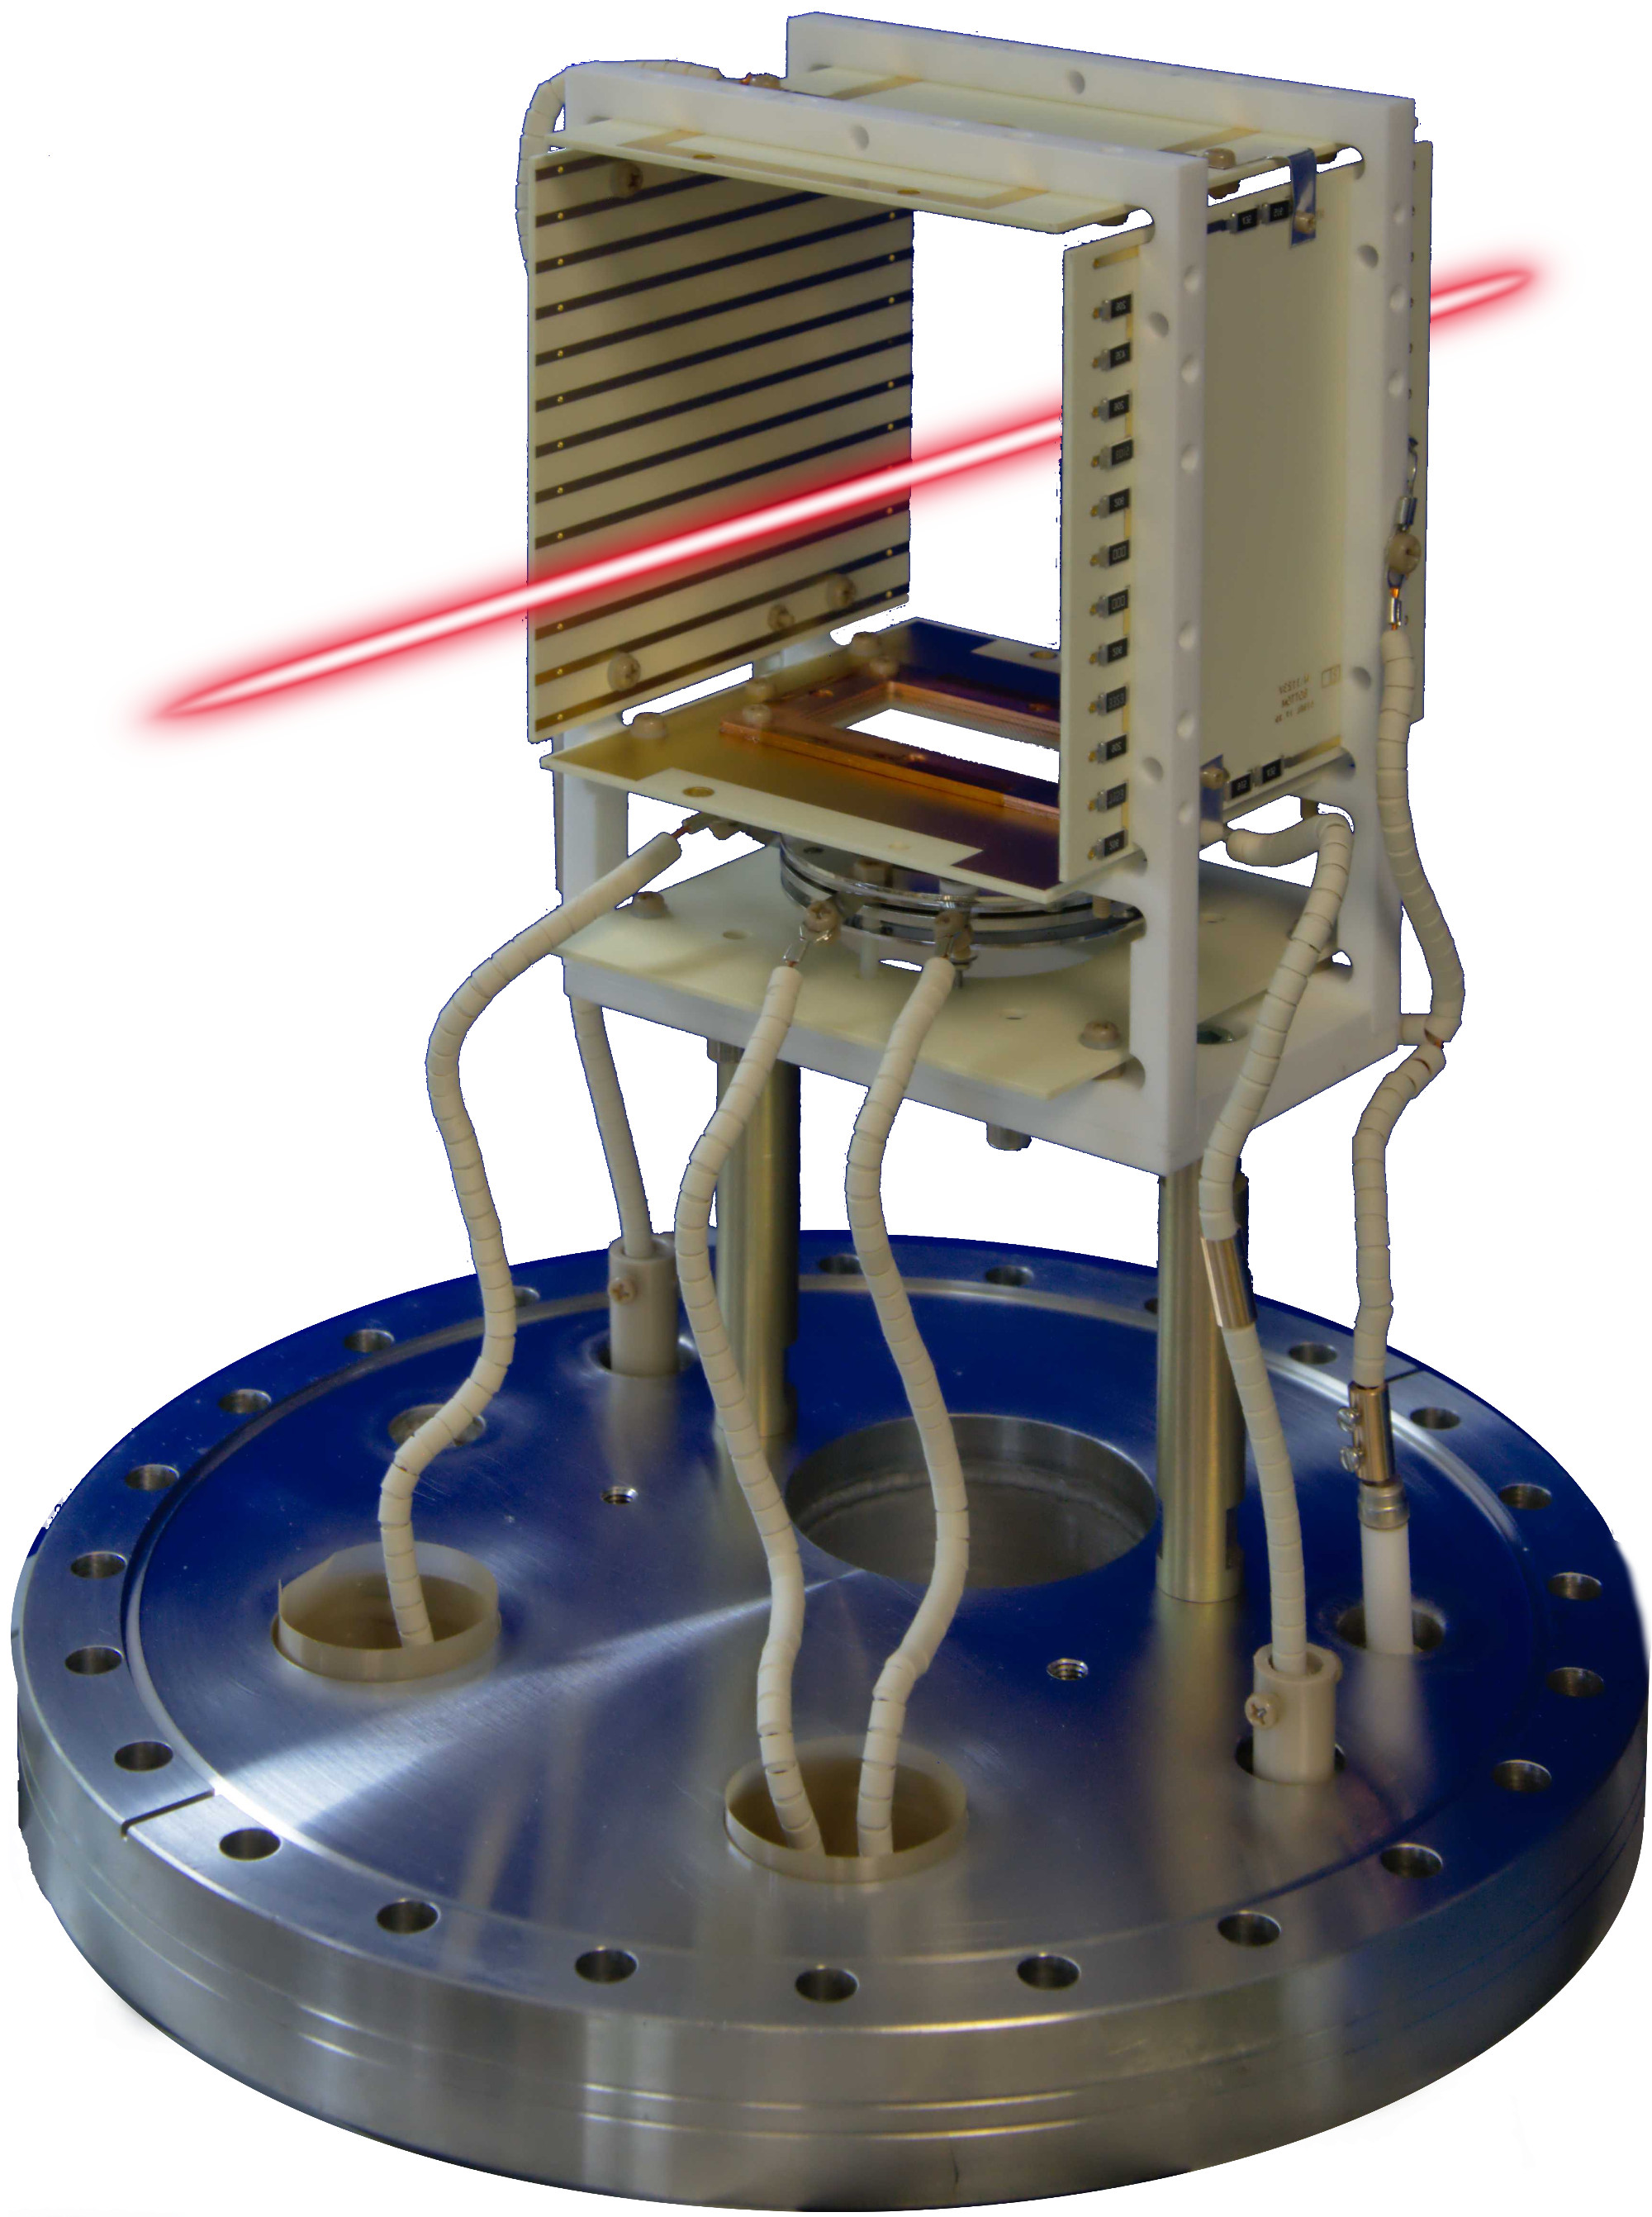
\includegraphics[width=3.5cm]{04_Test/fig/fig000_IPM_photo2}
    \end{textblock*}
    \begin{textblock*}{4.5cm}(7.25cm,6.25cm)      
      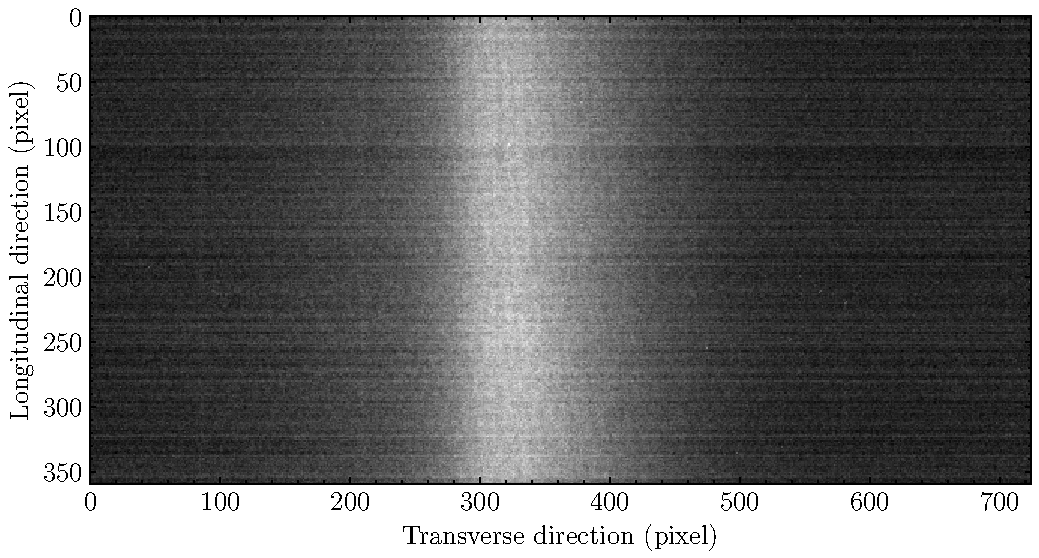
\includegraphics[width=4.5cm]{04_Test/fig/fig000_image_beam}
    \end{textblock*}
    % \begin{textblock*}{4cm}(8cm,6.5cm)      
    %   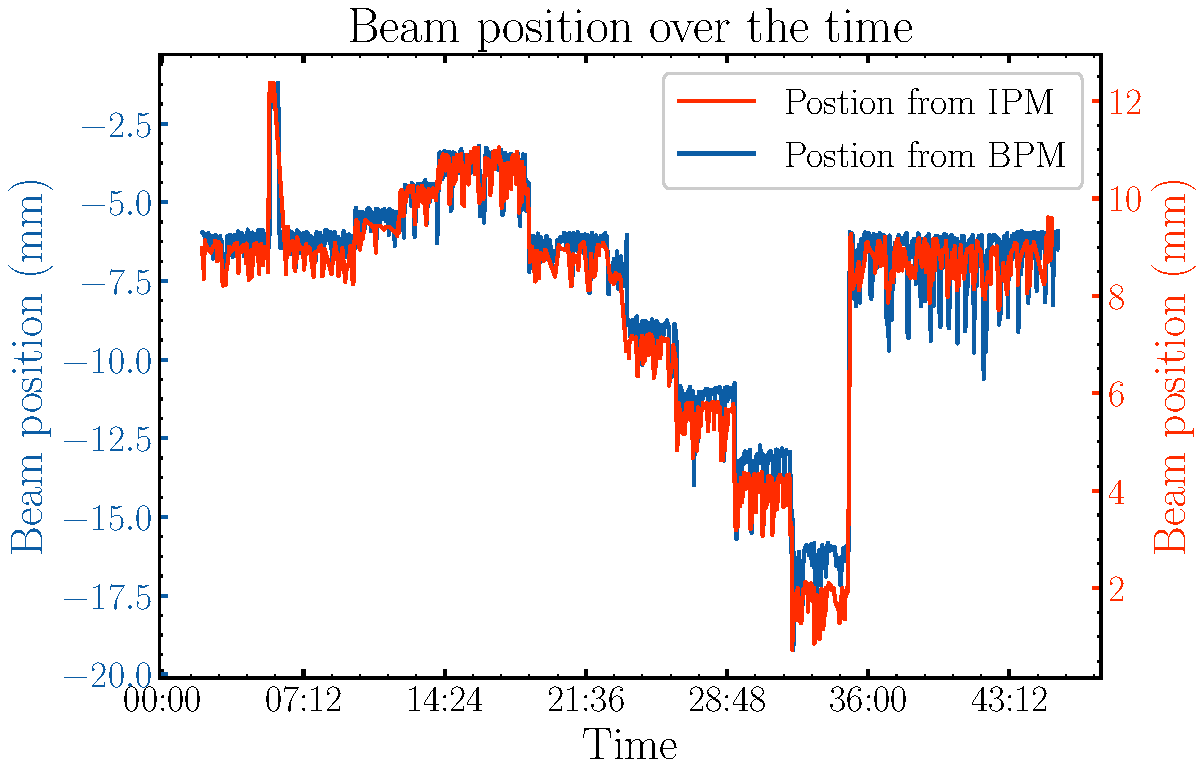
\includegraphics[width=4cm]{04_Test/fig/fig000_beam_car_a}
    % \end{textblock*}
\end{frame}

\begin{frame}[t]
  \frametitle{Beyond ESS}
  \begin{columns}[]
    \begin{column}{0.45\textwidth}
      \begin{block}{SONATE: a new compact neutron source}
        \begin{itemize}
          \item ILL + Orphée (LLB)
                \begin{itemize}
                  \item 94\% of instrument-day in France.
                  \item Closed in the next decade.
                \end{itemize}
          \item Accelerator driven source.
                \begin{itemize}
                  \item $20\,\mathrm{MeV}$ $100\,\mathrm{mA}$
                  \item Be target + Moderators
                \end{itemize}
        \end{itemize}
      \end{block}
    \end{column}
    \begin{column}{0.45\textwidth}
      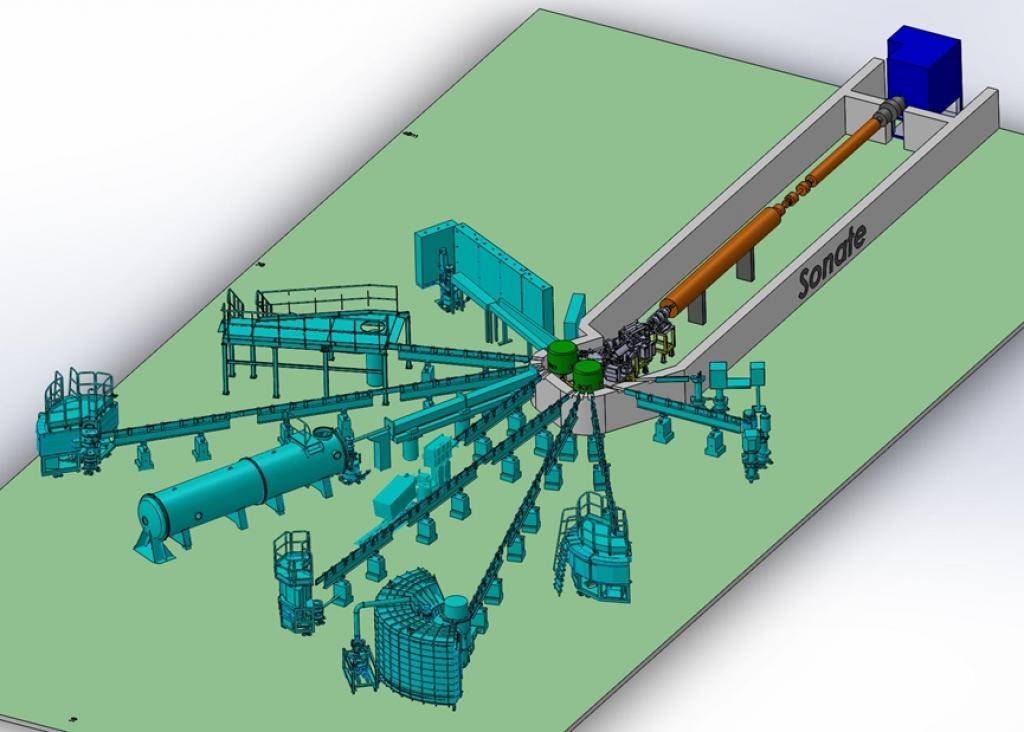
\includegraphics[width=1\textwidth]{05_Conclusion/fig/fig000_SONATE}
    \end{column}
  \end{columns}
  \begin{block}{IPHI is a key tool to validate the concept of SONATE.}
    A new collaboration has started to provide one IPM pair to IPHI, based on our prototypes.
  \end{block}
\end{frame}